\documentclass[]{article}
\usepackage[utf8]{inputenc}
\usepackage{parskip}
\usepackage{pdfpages}
\usepackage{amssymb}
\usepackage{stix}
\usepackage{hhline}
\usepackage{amsmath}
\usepackage{mathtools}
\usepackage{lipsum}
\usepackage{bm}
\usepackage[dvipsnames]{xcolor}
\usepackage{xspace}
\usepackage{multirow,tabularx}
\usepackage{siunitx}
%\usepackage{textgreek}
%\usepackage{upgreek}
\usepackage{multirow}
\usepackage{graphicx}
%\usepackage{pifont}
\usepackage{xstring}
\usepackage{etoolbox}
\usepackage{notoccite}
\usepackage{natbib}
%\usepackage{mathrsfs}
\usepackage{lineno}
\usepackage{tensor}
\usepackage[thinlines,thicklines]{easybmat}
%\usepackage{bbm}
\usepackage{accents}
\usepackage{tikz}

\DeclareSIUnit\parsec{pc} %define a parsec unit
\DeclareSIUnit\littleh{\mathsf{h}} %define normalised Hubble number
\DeclareSIUnit\ccs{{m_{\text{p}}}^2} %use of reduced Planck mass as unit
\DeclareSIUnit\nothing{\relax} %enable use of dimensionless quantities via siunitx package

\parskip 1mm
\parindent 2mm

%\newcommand{\simeq}{\mathrel{\smash[t]{\stackrel{{\text{an}}}{=}}}} %analogue equality
\newcommand{\ifeq}{\mathrel{\smash[t]{\stackrel{{\text{(e.g.)}}}{=}}}} %analogue equality
\newcommand{\og}{\bar{g}} %analogue equality
\newcommand{\feynman}{\tensor{D}{_{\text{F}}}} %Feynman propagator

\newcommand{\comment}[1]{\par {\sffamily  \color{red} #1 \par}} %for comments during editing


\usepackage{hyperref}
\hypersetup{%
     colorlinks = true,%
     linkcolor = Blue,%
     citecolor = Blue,%
     filecolor = Blue,%
     urlcolor = Blue% 
     }%
\usepackage[capitalize]{cleveref} %always load this last in preamble
\maxdeadcycles=1000

\begin{document}
%\setpagewiselikenumbers
%\modulolinenumbers[5]

\title{A mock}

%\date{}


%\pacs{04.50.Kd, 04.60.-m, 04.20.Fy, 98.80.-k}

\pagenumbering{gob}

\maketitle

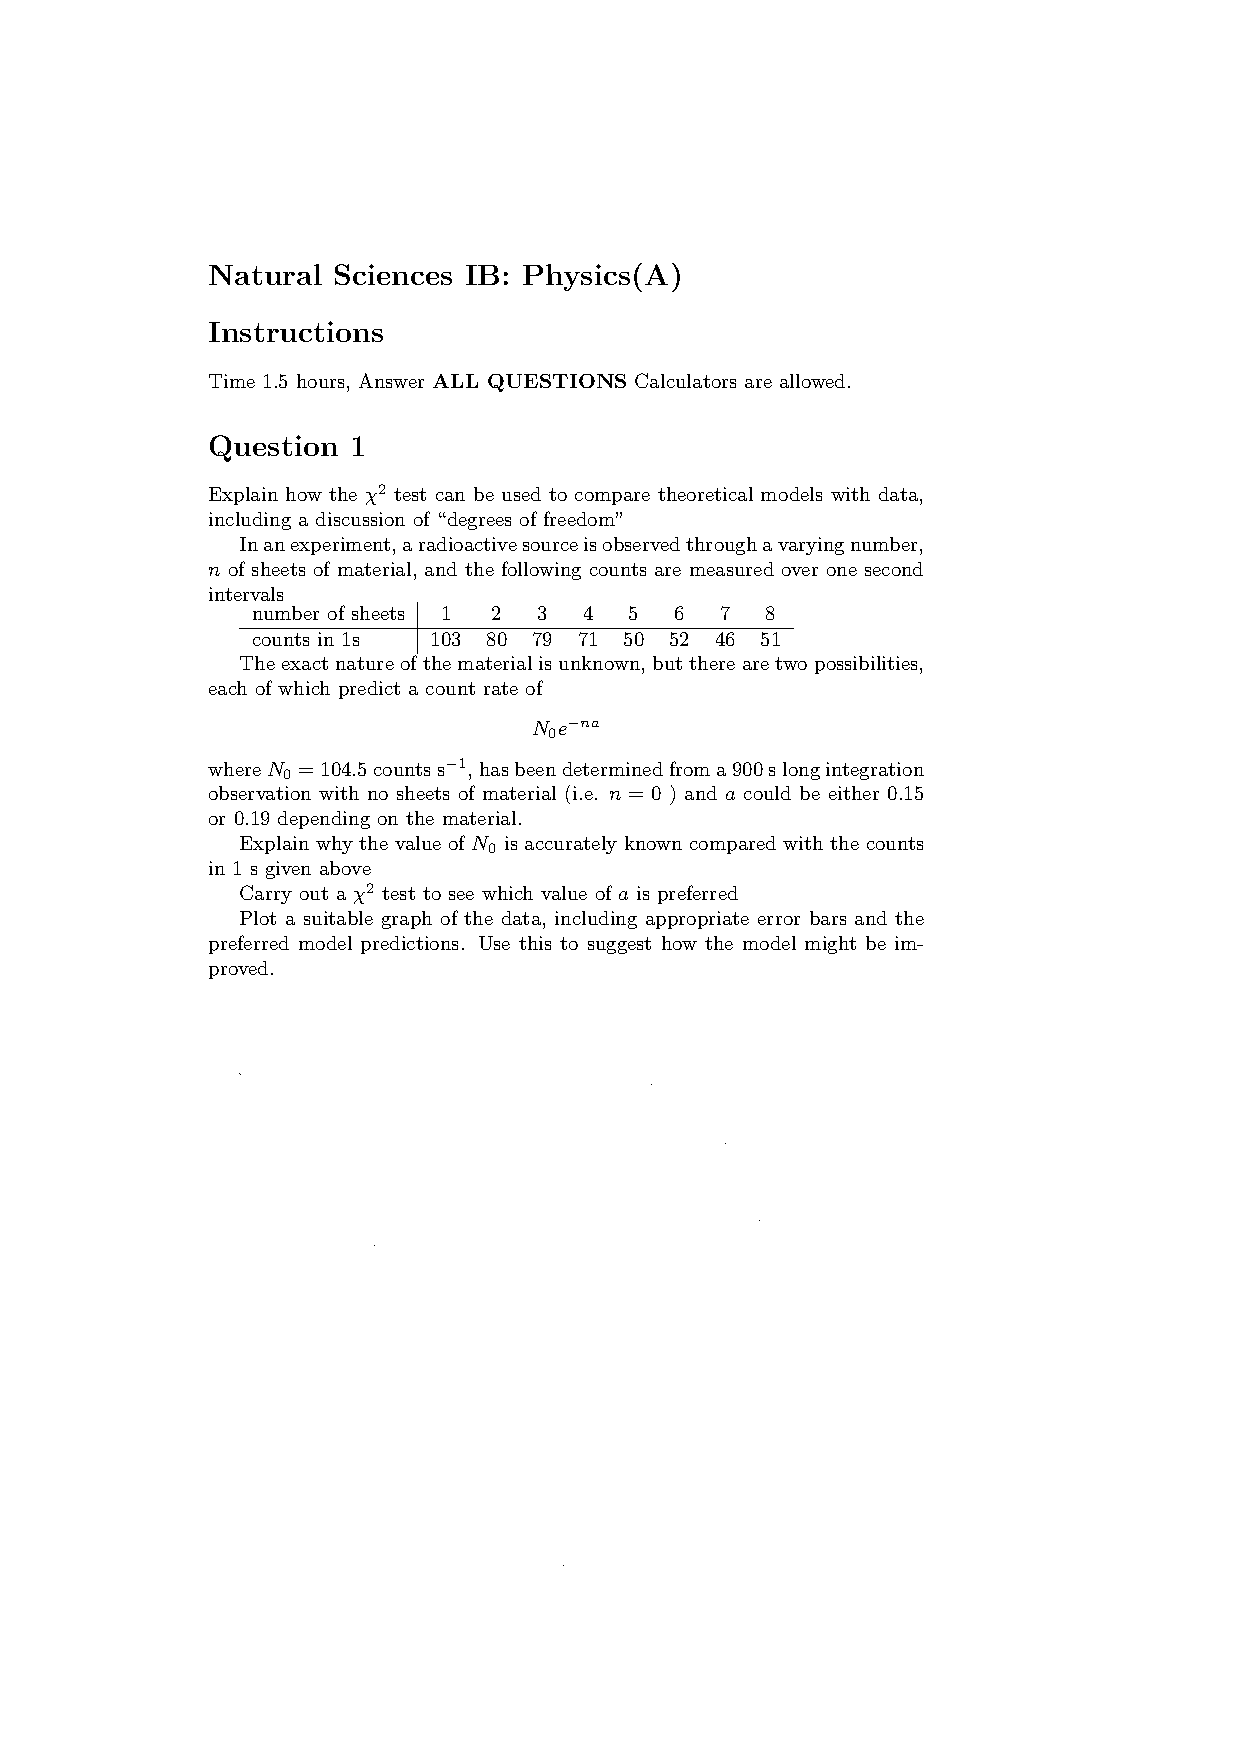
\includepdf[pages=1]{old2.pdf}


\section*{Question 2}

A neutral scalar field $\phi=\phi(x,y,t)$ lives on a half-infinite, flat $d=2$ strip with Cartesian coordinates ${0\leq x <\infty}$ and ${0\leq y\leq a}$ and evolves over time $t$ with equation of motion
\begin{equation*}
	\left(\partial^2_t-\partial^2_x-\partial^2_y\right)\phi=0.
\end{equation*}

The Dirichlet condition $\phi(x,0,t)=\phi(x,a,t)=0$ is now imposed. Derive the induced mass spectrum for relativistic particles propagating along the strip, as discussed in supervisions
\begin{equation*}
	m_n\equiv \frac{n\pi}{a}, \quad n\in \mathbb{N}.
\end{equation*}

The system is prepared in the ground state $\phi(x,y,-\infty)=0$, and at around $t=0$ an attempt is made to heat the system by imposing a further Dirichlet condition
\begin{equation*}
	\phi(0,y,t)=\mathfrak{R}\left\{e^{-(iE+\epsilon^2 t)t}f(y)\right\},\quad E,\epsilon,f(y) \in\mathbb{R},
	\quad \epsilon a\ll 1,
\end{equation*}
where $f(y)$ is a very noisy random function (e.g. white noise), and $f(0)=f(a)=0$. Discuss the condition on $E$ for substantial heating to occur.

At some $x_0\gg a$ a light particle is first observed at $t_0\gg a$, followed by a particle of twice the mass at $2t_0$. Infer $E$ in this case and explain why any other particles will be relatively hard to detect.

\includepdf[pages=2]{old2.pdf}

\end{document}
